\section{Assembling Single-end Reads}

The following exercise focuses on velvet using single-end reads, how the
available parameters effect an assembly and how to measure and compare the
changes.

\emph{Even though you have carefully compiled velvet in your own
workspace, we will be use the pre-installed version.}

\begin{note}
The data you will use is from Staphylococcus aureus USA300 which has a
genome of around 3MBases. The reads are unpaired Illumina, also known as
single-end library.

The data for this section was obtained from the Sequence Read Archive (SRA),
using \texttt{SRR022825} and \texttt{SRR022823} run data from SRA Sample
\texttt{SRS004748}. The SRA experiment can be viewed at:

\center{\url{http://www.ebi.ac.uk/ena/data/view/SRS004748}}

\end{note}

\begin{steps}
To begin with, first move back to the directory you prepared for this exercise,
create a new folder with a suitable name for this part and move into it. There
is no need to download the read files, as they are already stored locally.
Instead we will create symlinks to the files. Continue by copying (or typing):
\begin{lstlisting}
cd ~/NGS/velvet/part1
mkdir SRS004748
cd SRS004748
pwd
ln -s ~/NGS/Data/SRR022825.fastq.gz ./
ln -s ~/NGS/Data/SRR022823.fastq.gz ./
ls -l
\end{lstlisting}
\end{steps}

\begin{information}
You are ready to process your data with Velvet. There are two main components to
Velvet:
\begin{description}[style=multiline,labelindent=0cm,align=right,leftmargin=\descriptionlabelspace,rightmargin=1.5cm,font=\ttfamily]
  \item[velveth] Used to construct, from raw read data, a dataset organised in the
    fashion expected by the second component, \texttt{velvetg}.
  \item[velvetg] The core of velvet where the de Bruijn graph assembly is built and
    manipulated.
\end{description}

You can always get further information about the usage of both velvet programs
by typing \texttt{velvetg} or \texttt{velveth} in your terminal.
\end{information}

\begin{steps}
Now run \texttt{velveth} for the reads in \texttt{SRR022825.fastq.gz} and
\texttt{SRR022823.fastq.gz} using the following options:
\begin{itemize}
  \item A de Bruijn graph k-mer of 25
  \item An output directory called run\_25
\end{itemize}
\begin{lstlisting}
velveth run_25 25 -fastq.gz -short SRR022825.fastq.gz SRR022823.fastq.gz
\end{lstlisting}

\texttt{velveth} Once \texttt{velveth} finishes, move into the output directory
\texttt{run\_25} and have a look at what \texttt{velveth} has generated so far.
The command \texttt{less} allows you to look at output files (press \texttt{q}
to quit and return to the command prompt). Here are some other options for
looking at file contents:

\begin{lstlisting}
cd run_25
ls -l
head Sequences
cat Log
\end{lstlisting}

\end{steps}

\begin{questions}
What did you find in the folder \texttt{run\_25}?
\begin{answer}
Sequences, Roadmaps, Log
\end{answer}

Describe the content of the two \texttt{velveth} output files?
\begin{answer}
Sequences: FASTA file version of provided reads\\
Roadmaps: Internal file of velvet - basic information about number of reads, k-mer size
\end{answer}

What does the \texttt{Log} file store for you?
\begin{answer}
Time stamp, Executed commands; velvet version + compiler parameters, results
\end{answer}
\end{questions}

\begin{steps}
Now move one directory level up and run \texttt{velvetg} on your output directory, with
the commands:
\begin{lstlisting}
cd ../
time velvetg run_25
\end{lstlisting}

Move back into your results directory to examine the effects of \texttt{velvetg}:
\begin{lstlisting}
cd run_25
ls -l
\end{lstlisting}
\end{steps}

\begin{questions}
What extra files do you see in the folder \texttt{run\_25}?
\begin{answer}
PreGraph, Graph, stats.txt, contigs.fa, LastGraph
\end{answer}

What do you suppose they might represent?
\begin{answer}
PreGraph, Graph, LastGraph: Velvet internal graph representation at different
stages (see manual for more details about the file format)

stats.txt: tab-delimited description of the nodes of the graph incl. coverage information

contigs.fa: assembly output file
\end{answer}
  
In the Log file in \texttt{run\_25}, what is the N50?
\begin{answer}
4409 bp
\end{answer}
\end{questions}

\begin{information}
Hopefully, we will have discussed what the N50 statistic is by this point.
Broadly, it is the median (not average) of a sorted data set using the length of
a set of sequences. Usually it is the length of the contig whose length, when
added to the length of all longer contigs, makes a total greater that half the
sum of the lengths of all contigs. Easy, but messy - a more formal definition
can be found here:

\center{\url{http://www.broadinstitute.org/crd/wiki/index.php/N50}}
\end{information}

\begin{steps}
Backup the \texttt{contigs.fa} file and calculate the N50 (and the N25,N75) value with
the command:
\begin{lstlisting}
cp contigs.fa contigs.fa.0
gnx -min 100 -nx 25,50,75 contigs.fa
\end{lstlisting}

\end{steps}

\begin{questions}
Does the value of N50 agree with the value stored in the Log file?
\begin{answer}
No
\end{answer}

If not, why do you think this might be?
\begin{answer}
K-mer N50 vs bp N50; contig length cut-off value, estimated genome length
\end{answer}

\end{questions}

\begin{information}
In order to improve our results, take a closer look at the standard options of
\texttt{velvetg} by typing \texttt{velvetg} without parameters. For the moment
focus on the two options \texttt{-cov\_cutoff} and \texttt{-exp\_cov}. Clearly
\texttt{-cov\_cutoff} will allow you to exclude contigs for which the k-mer
coverage is low, implying unacceptably poor quality.
The \texttt{-exp\_cov} switch is used to give \texttt{velvetg} an idea of the
coverage to expect.

If the expected coverage of any contig is substantially in excess of the
suggested expected value, maybe this would indicate a repeat. For further
details of how to choose the parameters, go to ``Choice of a coverage cutoff'':

\center{\url{http://wiki.github.com/dzerbino/velvet/}}

\end{information}

\begin{steps}
Briefly, the k-mer coverage (and much more information) for each contig is stored
in the file \texttt{stats.txt} and can be used with R to visualize the k-mer coverage
distribution. Take a look at the \texttt{stats.txt} file, start R, load and
visualize the data using the following commands:
\begin{lstlisting}[style=R]
R --no-save --no-restore
install.packages('plotrix')
library(plotrix)
data <- read.table("stats.txt", header=TRUE)
weighted.hist(data$short1_cov, data$lgth, breaks=0:50)
\end{lstlisting}

A weighted histogram is a better way of visualizing the coverage information,
because of noise (lots of very short contigs). You can see an example output
below:
\end{steps}

% TODO Can't put figure environment within steps, note etc environment
\begin{figure}[H]
\centering
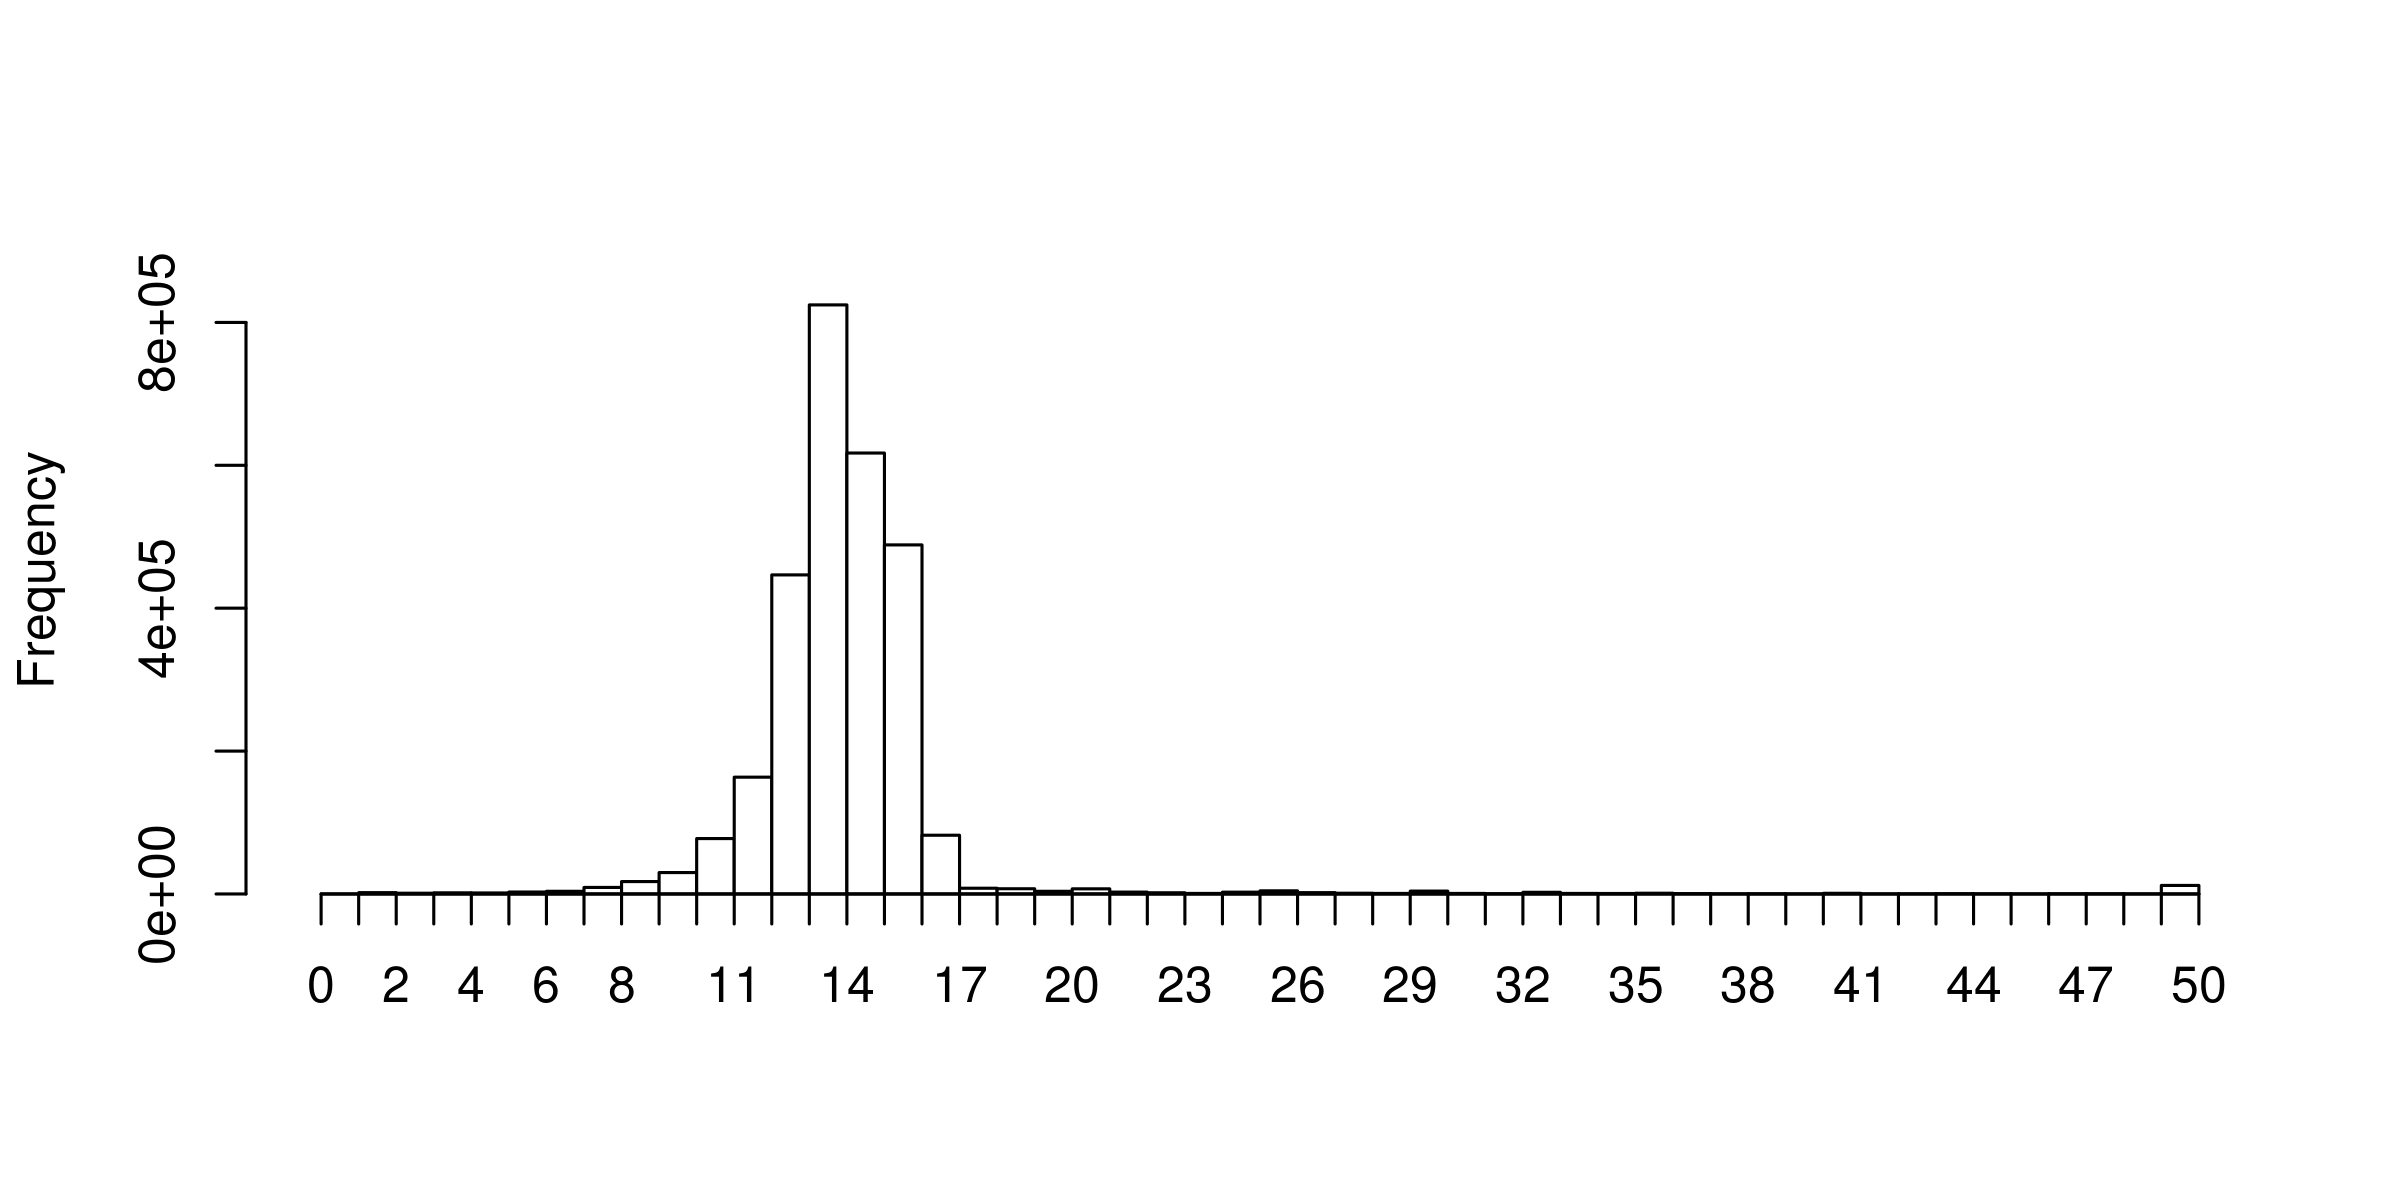
\includegraphics[width=0.8\textwidth]{de_novo/velvet/velvet_Rplot001.png}
\caption{\label{fig:SRS004748_coverage_hist} A weighted k-mer coverage histogram of the single-end reads.}
\end{figure}

\begin{steps}
After choosing the expected coverage and the coverage cut-off, you can exit R by
typing:
\begin{lstlisting}[style=R]
q()
\end{lstlisting}
\end{steps}

\begin{steps}
The weighted histogram suggests to me that the expected coverage is around 14
and that everything below 6 is likely to be noise. Some coverage is also
represented at around 20, 30 and greater 50, which might be contamination or
repeats (depending on the dataset), but at the moment this should not worry you.
To see the improvements, rerun \texttt{velvetg} first with \texttt{-cov\_cutoff} 6 and
after checking the N50 use only / add \texttt{-exp\_cov} 14 to the command line
option. Also keep a copy of the contigs file for comparison:
\begin{lstlisting}
cd ~/NGS/velvet/part1/SRS004748
time velvetg run_25 -cov_cutoff 6

# Make a copy of the run
cp run_25/contigs.fa run_25/contigs.fa.1

time velvetg run_25 -exp_cov 14
cp run_25/contigs.fa run_25/contigs.fa.2

time velvetg run_25 -cov_cutoff 6 -exp_cov 14
cp run_25/contigs.fa run_25/contigs.fa.3
\end{lstlisting}
\end{steps}

\begin{questions}
What is the N50 with no parameter:
\begin{answer}
4,447 bp
\end{answer}

What is the N50 with \texttt{-cov\_cutoff} 6:
\begin{answer}
5,168 bp
\end{answer}

What is the N50 with \texttt{-exp\_cov} 14:
\begin{answer}
4,903 bp
\end{answer}

What is the N50 with \texttt{-cov\_cutoff} 6 \texttt{-exp\_cov} 14:
\begin{answer}
5,417 bp
\end{answer}

Did you notice a variation in the time \texttt{velvetg} took to run? If so, can you
explain why that might be?
\begin{answer}
Velvet reuses already calculated results (from PreGraph,Graph)
\end{answer}

\end{questions}

\begin{steps}
You were running \texttt{velvetg} with the \texttt{-exp\_cov} and
\texttt{-cov\_cutoff} parameters. Now try to experiment using different
cut-offs, expected parameters and also explore other settings (e.g.
\texttt{-max\_coverage}, \texttt{-max\_branch\_length}, \texttt{-unused\_reads},
\texttt{-amos\_file}, \texttt{-read\_trkg} or see \texttt{velvetg} help menu).
\end{steps}

\begin{questions}
Make some notes about the parameters you've played with and the results you
obtained.
\begin{answer}
-max\_coverage: cut-off value for the upper range (like cov\_cutoff for the lower range)\\
-max\_branch\_length: length of branch to look for bubble\\
-unused\_reads: write unused reads into file\\
-amos\_file: write AMOS message file\\
-read\_trkg: tracking read (more memory usage) - automatically on for certain operations\\
\end{answer}
\\
\\
\\
\\
\end{questions}

\subsection{AMOS Hawkeye}

The \texttt{-amos\_file} argument tells \texttt{velvetg} to output the assembly
as an AMOS message file (\texttt{*.afg}) which can then be used by tools like
Hawkeye from the AMOS suite of tools.

\begin{steps}
Lets create the AMOS message file by running \texttt{velvetg} with some
appropriate parameters:
\begin{lstlisting}
velvetg run_25 -cov_cutoff 6 -exp_cov 14 -amos_file yes
\end{lstlisting}

\begin{note}
The \texttt{-exp\_cov} argument to enable read-tracking \texttt{-read\_trkg yes} in Velvet.
Without read tracking enabled, very little read-level information can be output
to the AMOS message file. This results in a pretty useless visualisation in
Hawkeye! However, since reads are being tracked, the analysis takes longer and
uses more memory.
\end{note}

Now convert the AMOS message file \texttt{velvet\_asm.afg} into an AMOS bank
using \texttt{bank-transact} and view the assembly with AMOS Hawkeye.
\begin{lstlisting}
bank-transact -c -b run_25/velvet_asm.bnk -m run_25/velvet_asm.afg
hawkeye run_25/velvet_asm.bnk
\end{lstlisting}

Have a look around the interface, in particular try to look at the ``Scaffold
View'' and ``Contig View'' of the larges scaffold. You should see something like
this:

\begin{figure}[H]
\centering
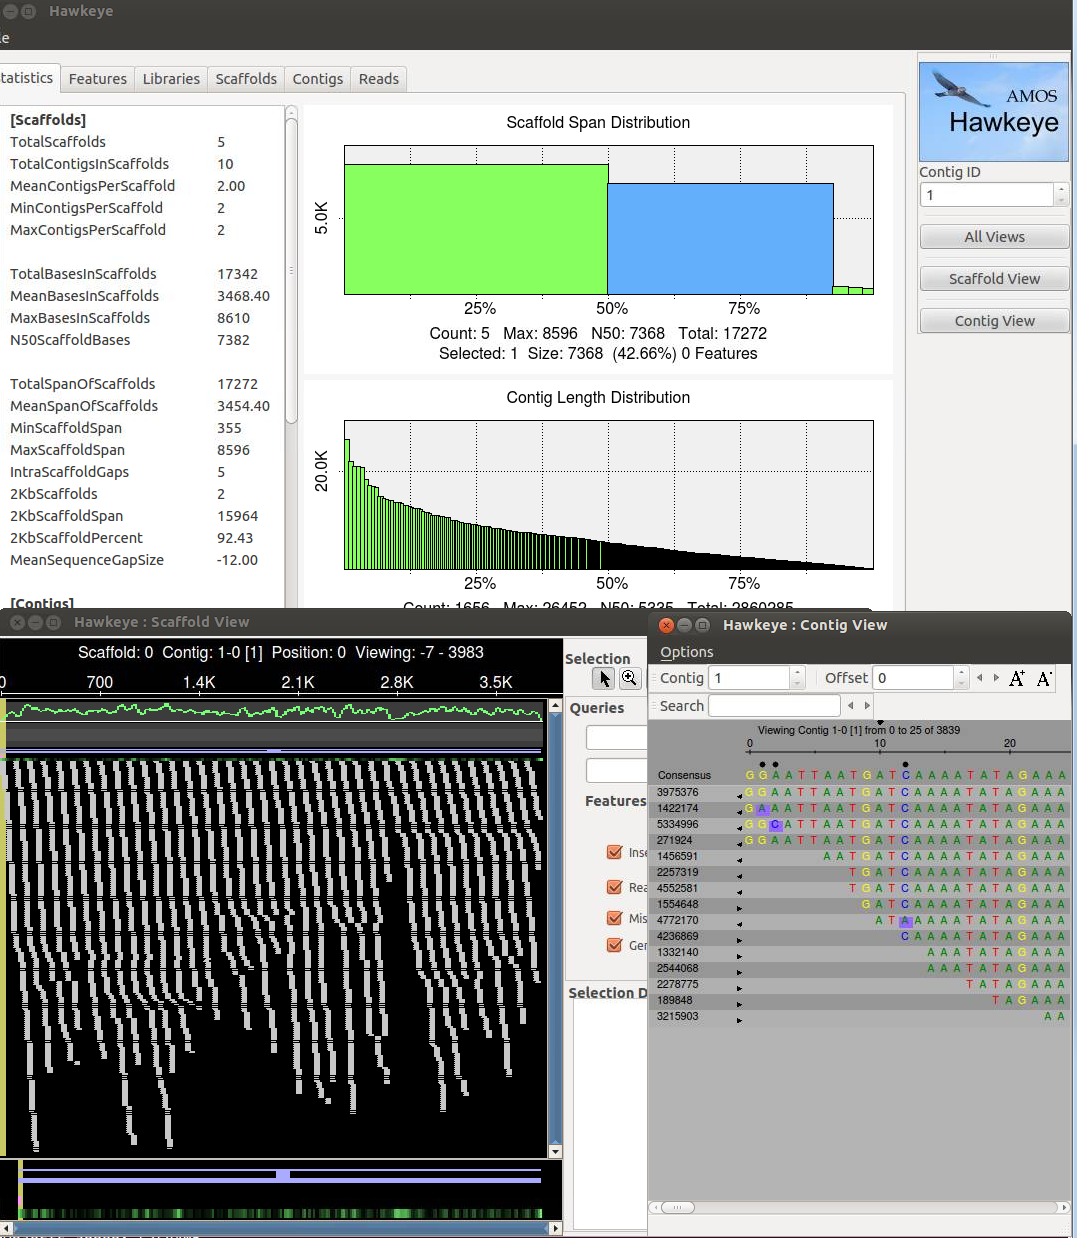
\includegraphics[width=0.8\textwidth]{de_novo/velvet/hawkeye_single_ended.png}
\caption{\label{fig:hawkeye_single_ended}}
\end{figure}

\end{steps}

\begin{bonus}
If you have time, try running the \texttt{velvetg} command without the
\texttt{-exp\_cov} argument, create the AMOS bank and see how the assemblies
look different in Hawkeye. Here's a hint:
\begin{lstlisting}
velvetg run_25 -cov_cutoff 6 -amos_file yes
bank-transact -c -b run_25/velvet_asm.bnk -m run_25/velvet_asm.afg
hawkeye run_25/velvet_asm.bnk
\end{lstlisting}

\end{bonus}

\begin{advanced}
\subsection{Simple Assembly Simulation}

\begin{note}
The data for this section is from Staphylococcus aureus MRSA252, a genome
closely related to the genome that provided the short read data in the earlier
sections of this exercise. The sequence data this time is the fully assembled
genome. The genome size is therefore known exactly and is 2,902,619 bp.
\end{note}

\begin{information}
In this exercise you will process the single whole genome sequence with \texttt{velveth}
and \texttt{velvetg}, look at the output only and go no further. The main intent of
processing this whole genome is to compute its N50 value. This must clearly be
very close to the ideal N50 value for the short reads assembly and so aid
evaluation of that assembly.
\end{information}

\begin{steps}
To begin, move back to the main directory for this exercise, make a
sub-directory for the processing of this data and move into it. All in one go,
this would be:
\begin{lstlisting}
cd ~/NGS/velvet/part1/ 
mkdir MRSA252 
cd MRSA252
\end{lstlisting}

Next, you need to download the genome sequence from
\url{http://www.ensemblgenomes.org/} which holds five new sites, for bacteria,
protists, fungi, plants and invertebrate metazoa. You could browse for the data
you require or use the file which we have downloaded for you. For the easier of
these options, make and check a symlink to the local file and with the
commands:
\begin{lstlisting}
ln -s ~/NGS/Data/s_aureus_mrsa252.EB1_s_aureus_mrsa252.dna.chromosome.Chromosome.fa.gz ./
ls -l
\end{lstlisting}

\end{steps}

\begin{note}
Usually Velvet expects relatively short sequence entries and for this reason has
a read limit of 32,767 bp per sequence entry. As the genome size is 2,902,619 bp
- longer as the allowed limit and does not fit with the standard settings into
velvet. But like the maximum k-mer size option, you can tell Velvet during
compile time, using \texttt{LONGSEQUENCES=Y}, to expect longer input sequences
than usual. I already prepared the executable which you can use by typing
\texttt{velveth\_long} and \texttt{velvetg\_long}.
\end{note}

\begin{steps}
Now, run \texttt{velveth\_long}, using the file you either just downloaded or created a
symlink to as the input:
\begin{lstlisting}
velveth_long run_25 25 -fasta.gz -long s_aureus_mrsa252.EB1_s_aureus_mrsa252.dna.chromosome.Chromosome.fa.gz
velvetg_long run_25
\end{lstlisting}

\end{steps}

\begin{questions}
What is the N50?
\begin{answer}
24,142 bp
\end{answer}

How does the N50 compare to the previous single end run (SRS004748)?
\begin{answer}
Big difference
\end{answer}
  
Does the total length differ from the input sequence length?
\begin{answer}
2,817,181 (stats) vs 2,902,619 (input)
\end{answer}
  
What happens when you rerun velvet with a different k-mer length?
\begin{answer}
K-mer 31: N50: 30,669 bp, total 2,822,878
\end{answer}

\end{questions}
\end{advanced}
